As platform, the KUKA youBot omni-directional mobile platform is used, which is equipped with a 5 DOF manipulator (Figure~\ref{fig:youBot}). At the end effector of the manipulator an Intel RealSense camera with a motion sensor is mounted. In order to improve grasping of more complex and bigger objects, the standard gripper has been replaced with a bigger gripper, made of soft material.   
%Next to the camera we replaced the standard gripper from youBot with an also youBots soft two-finger gripper. 
%Thanks to it we are able to grasp bigger and more complex objects more precisely.

A Hokuyo URG-04LX-UG01 laser scanner at the front of the youBot platform is used for localization and obstacle detection. 
%We are planning to add a second laser scanner of the same type on the back of the robot. This improves localization quality and ensures better obstacle avoidance, mainly when driving backwards with the robot. MOVED TO CONCLUSION (PHIL)
The controlling hardware consisted in 2015 of the internal computer of the youBot and an external ASUS Mini PC (4 GB RAM, Intel Core i3). The competition showed unfortunately, that this computer setup was not powerful enough, wherefore the CPU of the external computer has been replaced with a CPU Intel Core i7-4790K, 4x 4.00GHz. In order to avoid latencies between the computers, the internal PC of the youBot is mainly used to access the hardware of the robot such as the motors. Table~\ref{tab:hw} shows the current hardware specifications. \todo{fill in specs and format table}. 

%Last year we used the internal computer, together with an external ASUS Mini PC (4 GB RAM, Intel Core i3). We used the internal computer in the youBot to start-up the motors and also for the SLAM. This was a huge error because we added an enormous data transfer between the two computers, what slowed down the complete system. 

%To avoid the communication problems and latency between them both, we decided to run everything, except the motor drivers, on the external PC. We also replace the slow i3 for a more powerful CPU Intel Core i7-4790K, 4x 4.00GHz. Table~\ref{tab:hw} shows our new hardware specifications

A wireless LAN router is mounted on the robot, which on the one hand connects the two controlling computers. On the other hand, it creates a WLAN which allows easy remote access.

%For connecting the two PCs we use a router mounted on the back of youBot. With external machines we can connect to the routers network and communicate with both PCs on the youBot.

An Inertial Measurement Unit~(IMU) has been added to improve the localization. 
On the IMU runs a fusion algorithm which provides the orientation of the platform as quaternion or Euler angles.\todo{mit was wird hier fusioniert?!}

%We also added an Inertial Measurement Unit~(IMU) to gather information about the heading of the platform. On the IMU runs a fusion algorithm which provides the orientation of the platform as quaternion or Euler angles.

\begin{figure}[htbp]
	\begin{minipage}{0.45\textwidth}
		%\vspace{2.4cm}
		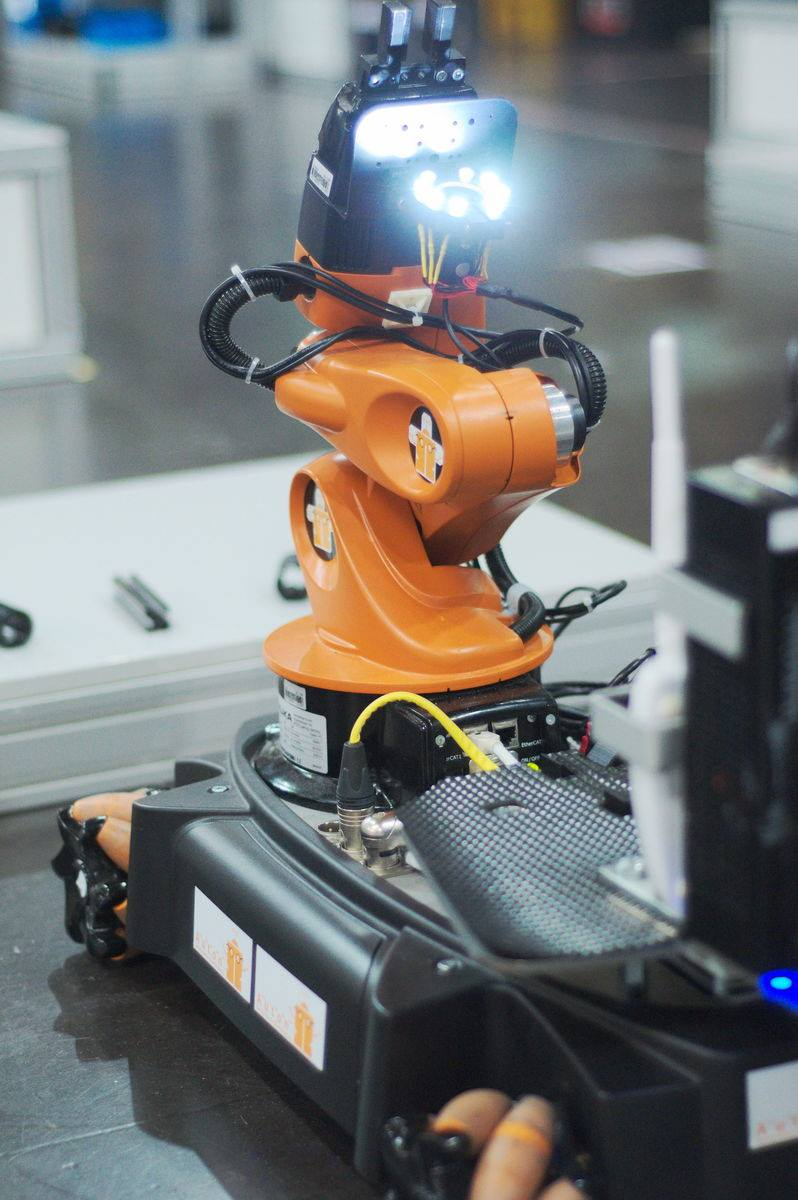
\includegraphics[width=\textwidth]{img/YoubotInAction.jpg}
		\caption{KUKA youBot Plattform}
		\label{fig:youBot}
	\end{minipage}
	\hfill
	\begin{minipage}{0.45\textwidth}
		\renewcommand*\figurename{Tab.}
		\setcounter{figure}{0}
		%	\begin{table}[htbp]
		\centering
		\caption{Hardware Specifications}
		\begin{tabular}{ | p{2cm} | p{3cm} | }
			\hline
			\bfseries{PC 1} &  \\
			\hline
			CPU & XXXXXXXX \\
			RAM & XXXXXXXX \\
			HDD & XXXXXXXX \\
			OS & Ubuntu 14.04 \\
			\hline \hline
			\bfseries{PC 2} &  \\
			\hline
			CPU & XXXXXXXX \\
			RAM & XXXXXXXX \\
			HDD & XXXXXXXX \\
			OS & Lubuntu 14.04 \\
			\hline \hline
			\bfseries{Grasp} &  \\
			\hline
			a & XXXXXXXX \\
			b & XXXXXXXX \\
			c & XXXXXXXX \\
			\hline \hline
			\bfseries{Lidar} &  \\
			\hline
			a & XXXXXXXX \\
			b & XXXXXXXX \\
			c & XXXXXXXX \\
			\hline \hline
			\bfseries{Router} &  \\
			\hline
			a & XXXXXXXX \\
			b & XXXXXXXX \\
			c & XXXXXXXX \\
			\hline \hline
			\bfseries{IMU} &  \\
			\hline
			a & XXXXXXXX \\
			b & XXXXXXXX \\
			c & XXXXXXXX \\
			\hline
		\end{tabular}
		\label{tab:hw}
	\end{minipage}
\end{figure}

\setcounter{figure}{1}

